\documentclass{article}

\usepackage{graphicx}
\usepackage{tikz}
\usepackage{tikzsymbols}
\usetikzlibrary{calc,patterns,shapes.geometric}
\pagestyle{empty}
\usepackage[margin=0pt]{geometry}
\geometry{papersize={14in,12in}}

\def\centerarc[#1](#2)(#3:#4:#5){\draw[#1] ($(#2)+({#5*cos(#3)},{#5*sin(#3)})$) arc (#3:#4:#5);}

\begin{document}
	\begin{figure}
		\centering
		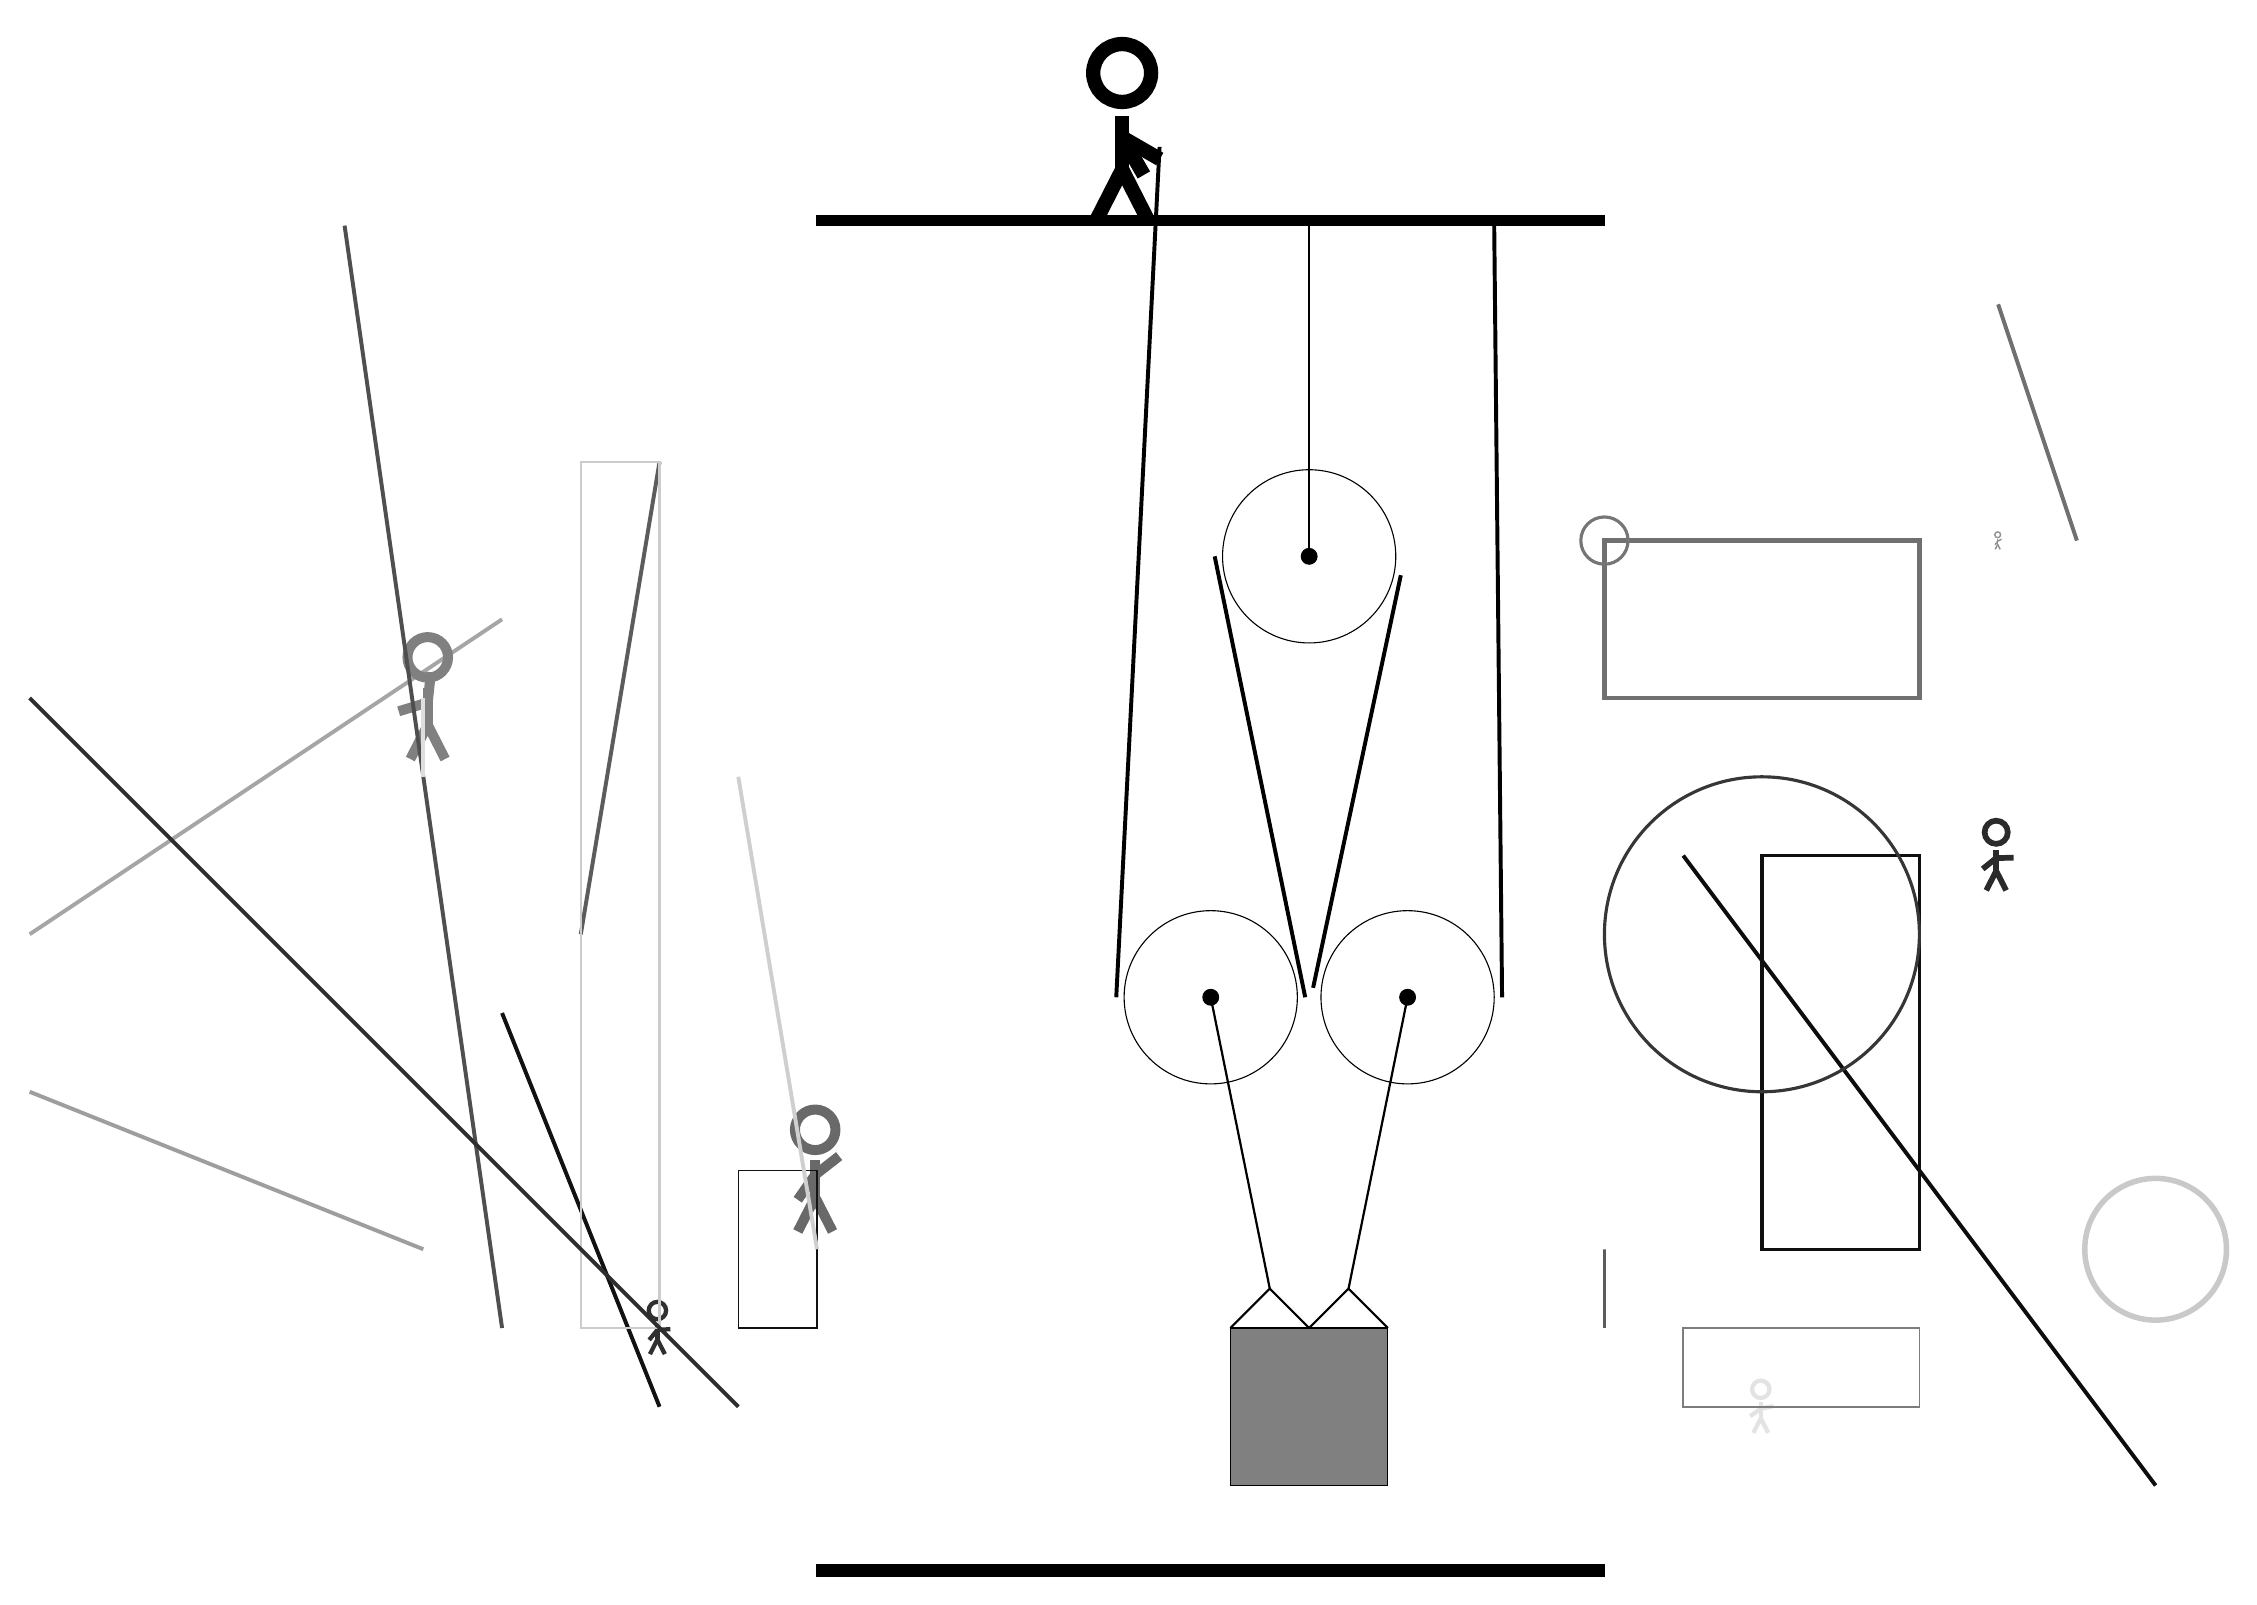
\begin{tikzpicture}
			%%%%% START %%%%%
			
			\draw[fill=black] (-4, 14) rectangle (6, 14.125);
			
			\draw (1, 4.2) circle (1.1);
			\draw[fill=black] (1, 4.2) circle (0.1);
			
			\draw (2.25, 9.8) circle (1.1);
			\draw[fill=black] (2.25, 9.8) circle (0.1);
			\draw[thick] (2.25, 9.8) -- (2.25, 14);
			
			\draw (3.5, 4.2) circle (1.1);
			\draw[fill=black] (3.5, 4.2) circle (0.1);
			
			\draw[thick] (3.5, 4.2) -- (2.75, 0.5);
			\draw[thick] (1, 4.2) -- (1.75, 0.5);
			\draw[thick]  (1.25, 0) -- (1.75, 0.5) -- (2.25, 0);
			\draw[thick]  (2.25, 0) -- (2.75, 0.5) -- (3.25, 0);
			\draw[fill=black!50] (1.25, 0) rectangle (3.25, -2);
			
			\node[line width=0.5mm, color=black!43] at (11, 10) {\Strichmaxerl[1][53][28]};
			
			\node[line width=0.6mm, color=black!81] at (-6, 0) {\Strichmaxerl[3][51][3]};
			\draw[line width=0.6mm, color=black!56] (6, 8) rectangle (10, 10);
			\node[line width=0.5mm, color=black!11] at (8, -1) {\Strichmaxerl[3][36][11]};
			
			\draw[line width=0.5mm, color=black!95](7, 6) -- (13, -2);
			\draw [line width=0.3mm, color=black!39](9, 7) circle (0.0);
			\draw[line width=0.5mm, color=black!35](-8, 9) -- (-14, 5);
			\draw [line width=0.4mm, color=black!54](6, 10) circle (0.3);
			\draw[line width=0.5mm, color=black!56](11, 13) -- (12, 10);
			
			\draw[line width=0.4mm, color=black!94] (8, 6) rectangle (10, 1);
			\node[line width=0.7mm, color=black!83] at (11, 6) {\Strichmaxerl[4][39][1]};
			
			\node[line width=0.2mm, color=black!50] at (-9, 8) {\Strichmaxerl[7][17][84]};
			\node[line width=0.5mm, color=black!59] at (-4, 2) {\Strichmaxerl[7][55][38]};
			
			\draw[line width=0.5mm, color=black!64](-7, 5) -- (-6, 11);
			\draw[line width=0.2mm, color=black!93] (-5, 0) rectangle (-4, 2);
			\draw[line width=0.5mm, color=black!93](-8, 4) -- (-6, -1);
			\draw[line width=0.5mm, color=black!69](-8, 0) -- (-10, 14);
			\draw [line width=0.4mm, color=black!79](8, 5) circle (2.0);
			\draw [line width=0.7mm, color=black!21](13, 1) circle (0.9);
			\draw[line width=0.2mm, color=black!51] (7, -1) rectangle (10, 0);
			\draw[line width=0.5mm, color=black!19](-4, 1) -- (-5, 7);
			
			\draw[line width=0.3mm, color=black!20] (-6, 0) rectangle (-7, 11);
			\draw[line width=0.3mm, color=black!64] (6, 1) rectangle (6, 0);
			\draw[line width=0.5mm, color=black!13](-9, 8) -- (-9, 7);
			\draw[line width=0.5mm, color=black!38](-9, 1) -- (-14, 3);
			\draw[line width=0.5mm, color=black!82](-5, -1) -- (-14, 8);
			
			
			\draw[line width=0.5mm] (0.35, 15) --  (-0.2, 4.2);
			\centerarc[line width=0.5mm](1, 4.2)(180:360:1.2000000000000002);
			\draw[line width=0.5mm] (2.2, 4.2) -- (1.05, 9.8);
			\centerarc[line width=0.5mm](2.25, 9.8)(-20:180:1.2000000000000002);
			\draw[line width=0.5mm](3.414, 9.56) -- (2.3, 4.32);
			\centerarc[line width=0.5mm](3.5, 4.2)(160:360:1.2000000000000002);
			\draw[line width=0.5mm](4.7, 4.2) -- (4.6, 14);
			
			\node at (-0.07, 15.2) {\Strichmaxerl[10][120][-30]};
			
			\draw[fill=black] (-4, -3) rectangle (6, -3.15);
			
			%%%%% END %%%%%
		\end{tikzpicture}
	\end{figure}	
\end{document}